El valor del par\'ametro U de Hubbard debe ser calculado para cada material estudiado. Un posible m\'etodo es el semiemp\'irico que consiste en probar varios valores del par\'ametro U hasta ajustar los resultados a datos experimentales del material. 
Un m\'etodo m\'as preciso para calcular el par\'ametro U de Hubbard es el m\'etodo de respuesta lineal, el cual se describe a continuaci\'on y fue el m\'etodo usado en este trabajo.

\subsection{M\'etodo de respuesta lineal}

El m\'etodo de respuesta lineal fue propuesto por Cococcioni y Gironcoli en el a\~no 2005 \cite{cococcioni2005}. Este m\'etodo consiste en realizar peque\~nas perturbaciones en la energ\'ia de los orbitales {\bf d}. Para medir la respuesta del sistema a las perturbaciones el m\'etodo propone estudiar el cambio de las ocupaciones de los orbitales {\bf d} respecto a las perturbaciones. En el m\'etodo el par\'ametro U se expresa de la siguiente forma.

\begin{equation}
    U = \chi _{0}^{-1} - \chi ^{-1} \textup{ ,}
\end{equation}

\noindent que toma en cuenta la energ\'ia asociada al cambio de una poblaci\'on de electrones y la energ\'ia asociada al cambio en otro estado, donde $\chi_{0}$ y $\chi$ se definen como

\begin{equation}
    \chi = \frac{dn}{d\alpha}
    \label{definicion_chi}
\end{equation}

\noindent Las perturbaciones deben ser peque\~nas y los valores tomados se encuentran normalmente alrededor de cero. Esto se aplicara a los electrones en estado {\bf d} ya que se espera un cambio de energ\'ia significativo por estar alejados del n\'ucleo.

\noindent Para utilizar este m\'etodo con Quantum ESPRESSO, se deben seguir los siguientes pasos. Primero se realiza un c\'alculo autoconsistente sin ning\'un tipo de perturbaci\'on, cuya soluci\'on autoconsistente ser\'a tomada como punto de partida para los siguientes c\'alculos. Luego se realizan c\'alculos autoconsistentes separados para cada valor de $\alpha $ considerado. En cada uno de estos c\'alculos se debe guardar el valor de la ocupaci\'on en la primera iteraci\'on y en la \'ultima iteraci\'on cuando alcanza la convergencia, lo cual son resultados accesibles en el programa.
Si graficamos las ocupaciones respecto de las perturbaciones obtenemos una gr\'afica como la siguiente \ref{RespuestaLineal}.


\begin{figure}[H]
    \centering
    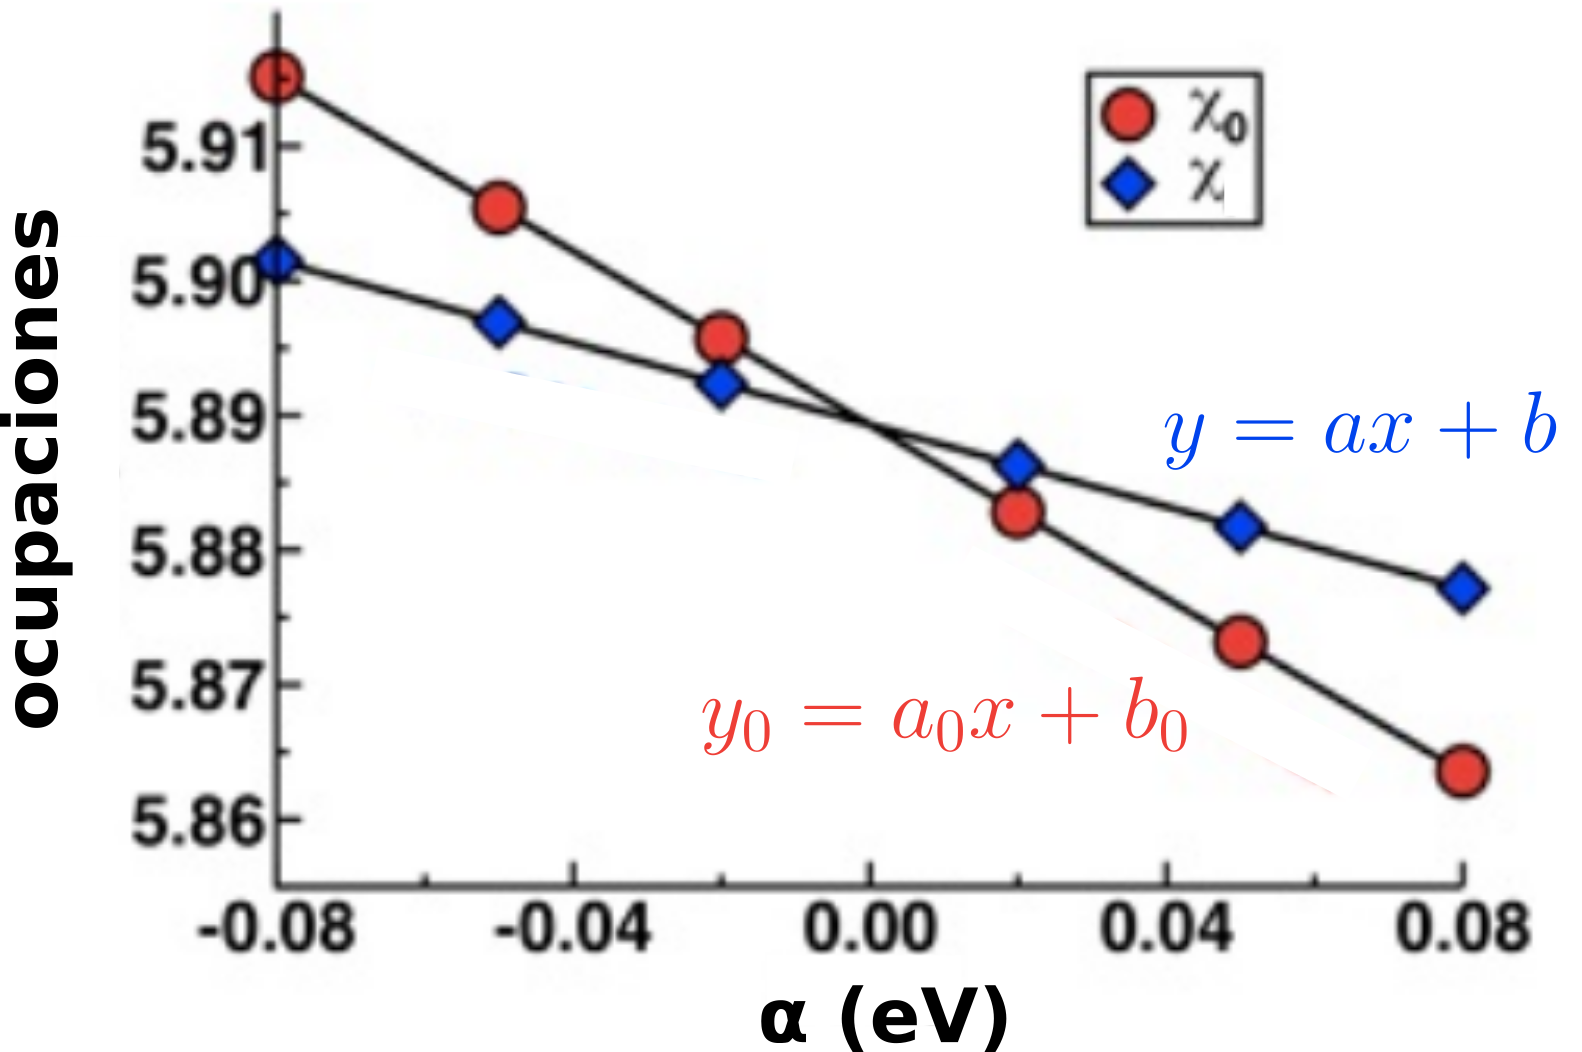
\includegraphics[width=0.6\linewidth]{contenido/calculos_computacionales/calculo_hubbard/img_lineal/RespuestaLineal}
    \caption{Ocupaciones versus perturbaciones.}
    \label{RespuestaLineal}
\end{figure}

\noindent La derivada \ref{definicion_chi} da el valor de $\chi_{0}$ y $\chi$ debe ser evaluada num\'ericamente, en este caso su valor es la pendiente de la recta correspondiente a $\chi_{0}$ o $\chi$. Refiri\'endonos  a la gr\'afica \ref{RespuestaLineal} el valor de $\chi_{0}$ es la pendiente de la recta de puntos rojos y el valor de $\chi$ es la pendiente de la recta de puntos azules.